

\subsection{LED controller}
The LEDs are used to detect the color of the brick by shining light onto the bricks and depending on the light intensity reflected, the system will know which color the passing brick has.
To do this the LEDs need to be controlled from the FPGA in order to turn on one of the LED colors at a time.
Since the LEDs are powered by a 12V supply then a driver for the LED is needed. 

It was decided to use a MOSFET transistor to drive the LEDs. 
This type of transistor allow us to turn on and off the LEDs with a output signal from the FPGA using a minimum current from the integrated circuit at high frequencies.

The selected transistor for this driver has been a NTD5867NL. 
This n-Channel MOSFET is able to drive up to 60V and 20A with a gate-to-source threshold voltage of 2.5V, which makes it perfect to drive the LEDs with a FPGA signal.
Apart from that, these MOSFET have a drain-to-source resistance of up to 50 m$\Omega$ (which can be ignored), and can be driven at speeds up to 30MHz.

In this project the LEDs are going to be turned on and off with a frequency of at most 170kHz, due to the sampling speed from the ADC, so the MOSFET is fast enough for this application.

In figure \ref{fig:LED_driver_sch} the schematics for the LED drivers are shown.

The selected LED colors for this project has been red, green and blue. 
Using the information given by the manufacturer and testing the intensities measured by the photodiode for the three brick colors, the current limiting resistor for the LEDs was chosen. 
The selected resistors is 1k$\Omega$ for the blue and green color and 430$\Omega$ for the red one.

\begin{figure}[H]
\centering 
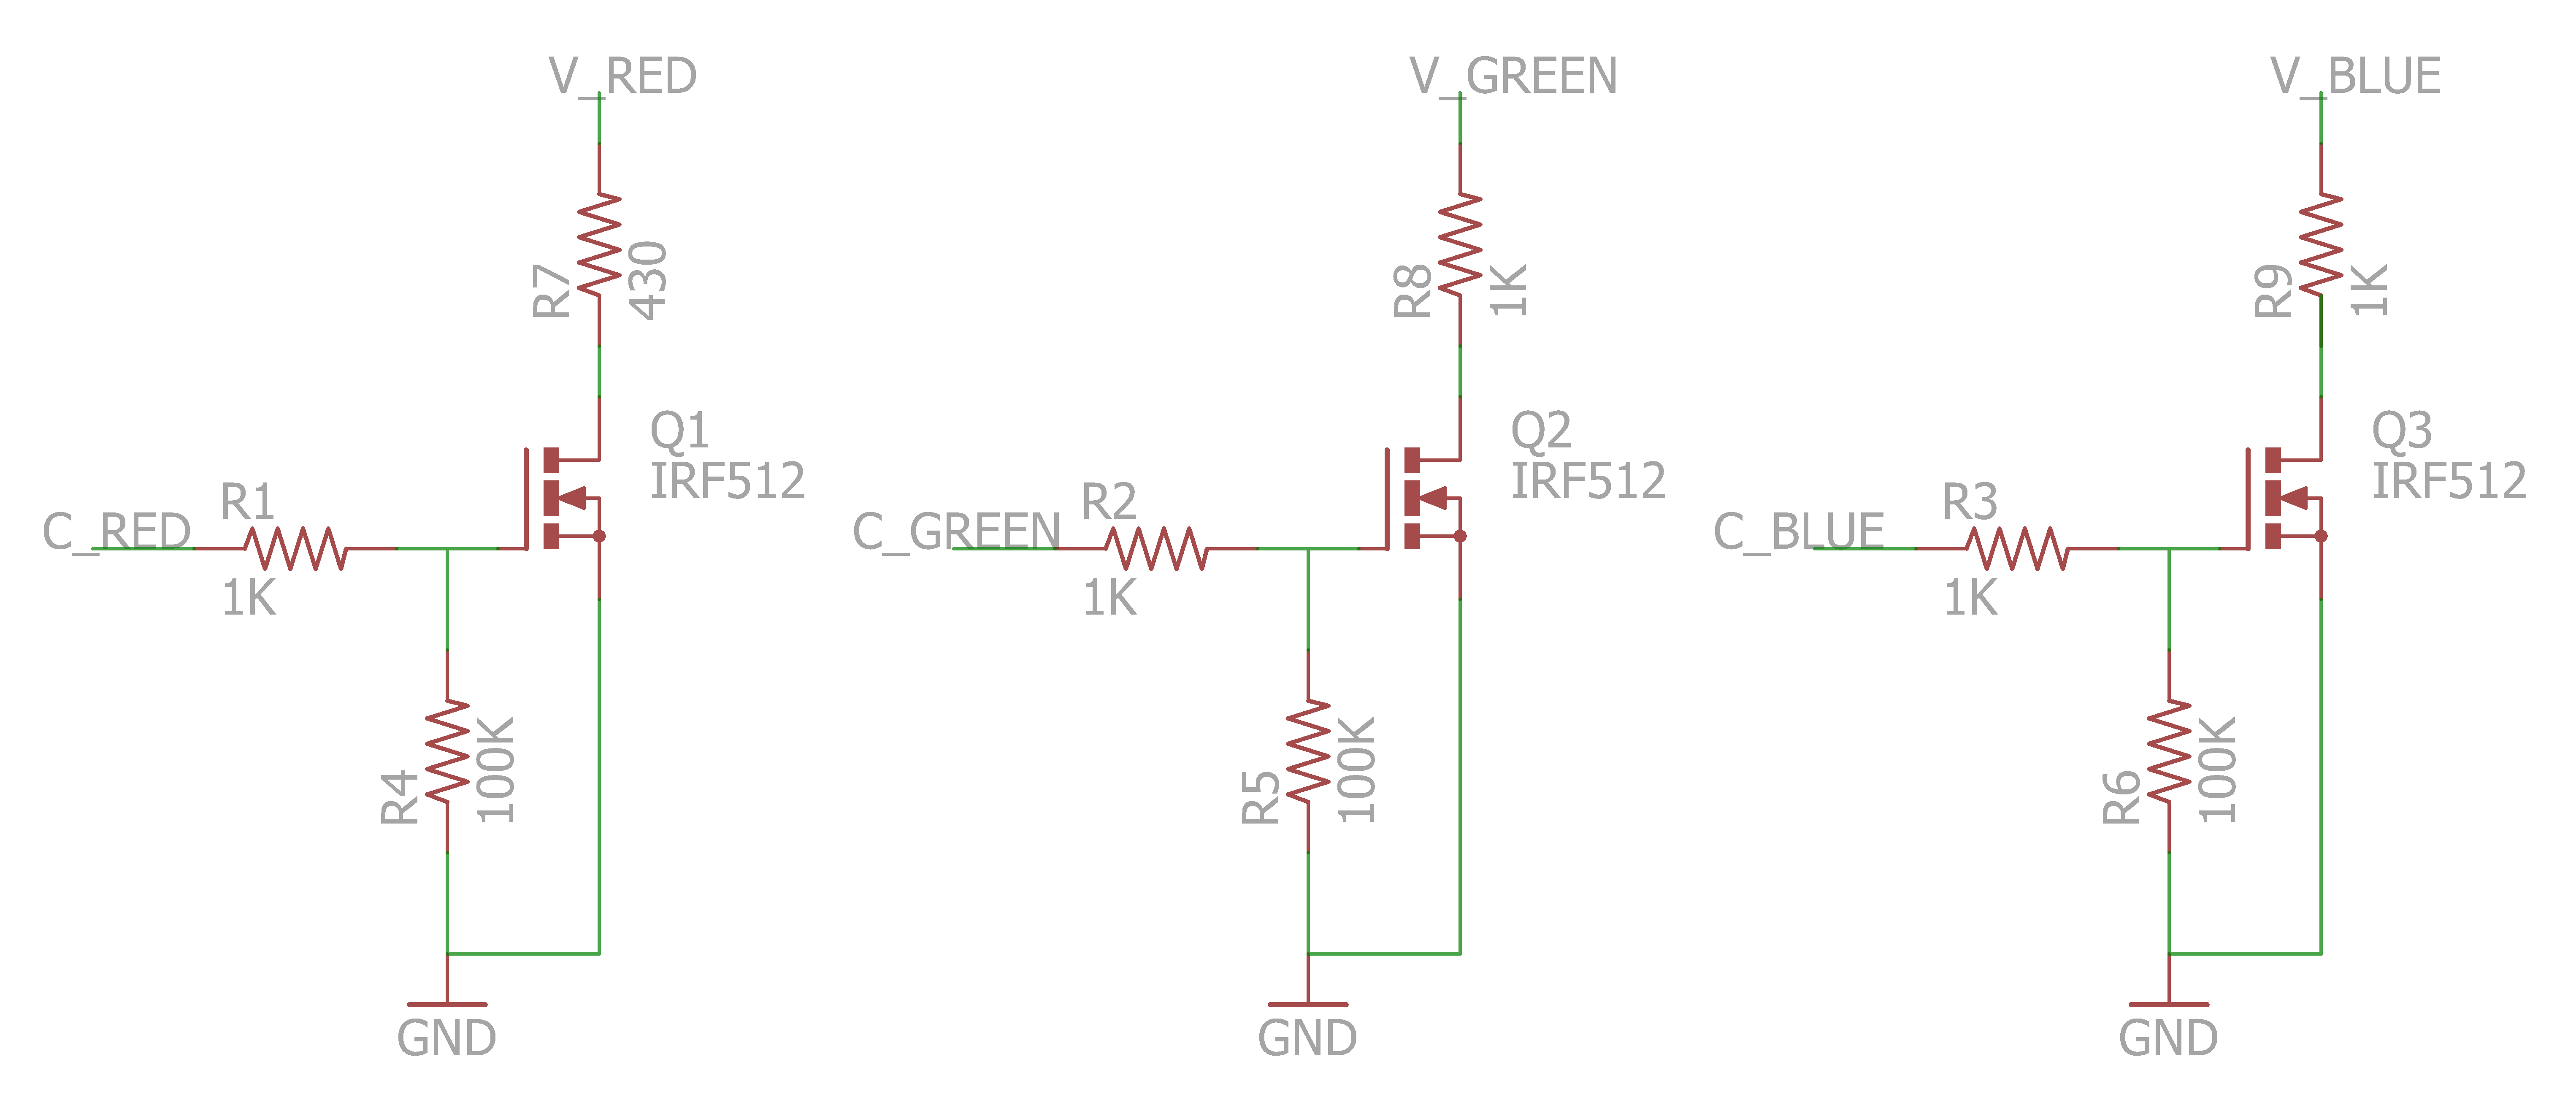
\includegraphics[width = 0.7 \textwidth]{images/leddriver_schematics}
\caption{LED driver schematics.}
\label{fig:LED_driver_sch}
\end{figure}


Given the resistances used, then the LEDs will at most be driven with 14mA.
This enables continuous lighting of the LEDs without breaching the recommended operation range of them.
It was also found that driving them with the given current is supplying sufficient light for the photodiode as considered in section \ref{sec:photodiode}.


It is however noticeable that the LEDs also could have been driven with a higher current.
This should decrease the amplification needed for the photodiode and hence increase the bandwidth of the amplifier.
Furthermore, the signal-to-noise ratio should be reduced on the photodiode because the intensity of the photodiode caused by the LEDs should be that much higher.
It was however still chosen to keep the selected resistances to maintain a longer lifetime of the LEDs and reduce the power consumption of the system.

